

\chapter{Prototype System}
The prototype system is the realisation of our conceptual model for reactive Information Systems and their services.
During our research we identified asynchronous communication and event-driven architecture (\textrm{EDA}) as necessary key properties for a reference implementation of our conceptual model.
Therefore we decided to rely on the recent adoption of JavaScript to application development, which is made possible through \textrm{Node.js}.
We believe in the future success of \textrm{JavaScript} for application development because the key concepts of asynchronous communication and non-blocking I/O are important properties for todays large scale applications.
Another advantage of this technology is the human-readable \textrm{JavaScript Object Notation} (\textrm{JSON}) for data exchange.
\textrm{JSON} builds only on two data structures:
\begin{itemize}
	\item Object: An unordered collection of name/value pairs, which can also be implemented as a hash map, dictionary or struct.
	\item Array: An ordered list of values, which can also be implemented as a record, vector or list.
\end{itemize}
A value can be an object or an array, but also a unicode string, a number, boolean or null.
This allows for any arbitrary depth and chaining of the supported data representations.
Since all data within JavaScript programming code is already in JSON format, it can easily be marshalled into one string and communicated to other applications without overhead.
Since \textrm{JSON} can be implemented in virtually every programming language, it received a lot of attention and is supported by many modern Web resources.

The prototype consists of a queue which receives all incoming events, and an engine that picks the events from the end of the queue whenever it is idle.
The engine checks the event against its stored ECA rules and fires the actions whenever a rule applies to an event.
When a new rule is stored, the engine instantiates the action modules that are required in case an event arrives at the system which triggers the actions.
The Web is a heterogeneous resource with many different types of systems and services, thus we can't rely on them for providing events to the webhooks of our system.
Thus we also implement the so called "event triggers" a way to pull events into our system through.
All they do is checking Web resources for changes and push events into the system whenever they detect one.
\begin{figure}[!ht]
	\centering
  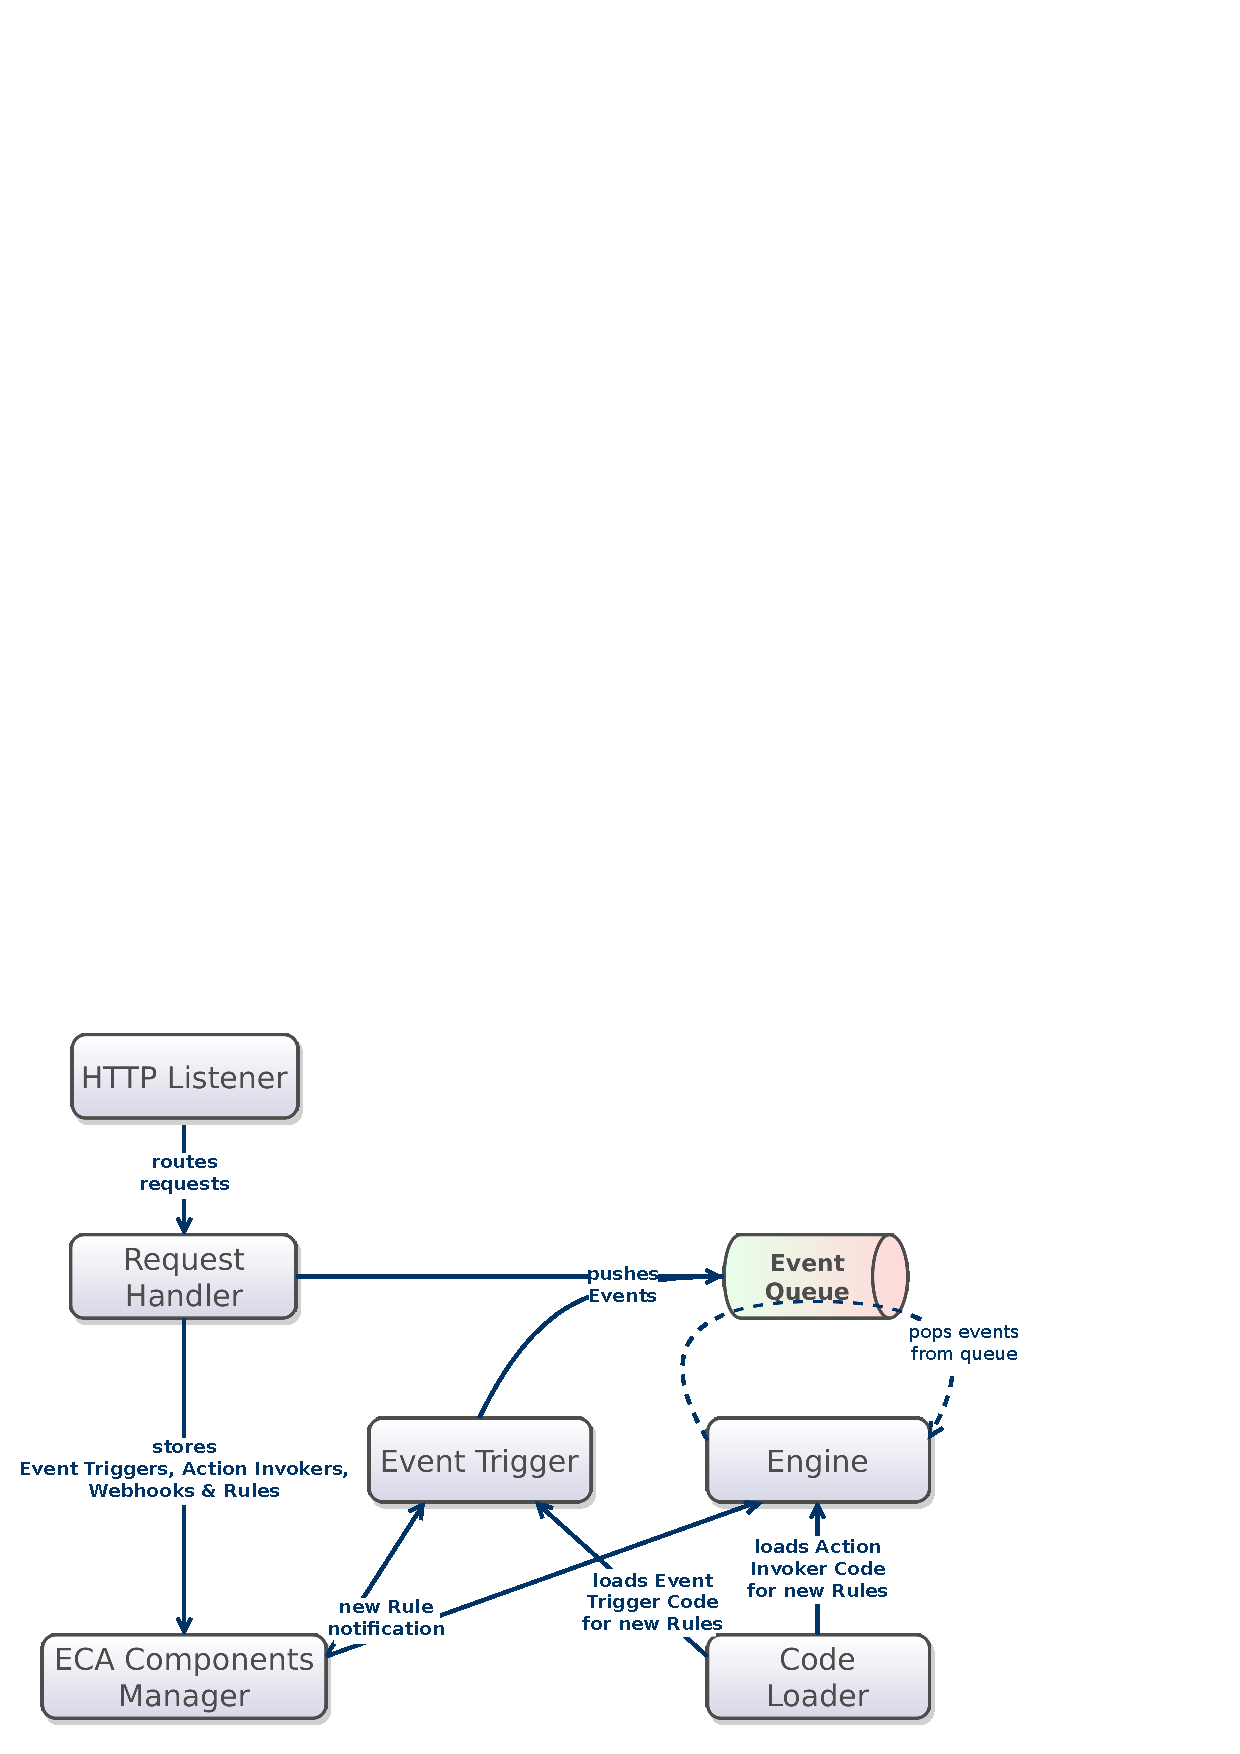
\includegraphics[width=0.9\textwidth]{figures/Architecture_wET}
	\caption{Prototype Process diagram}
	\label{fig:Architecture_wET}
\end{figure}

% There's still the challenge of filtering
% What's important to whom
% Plus the user needs to have tools to combine and add programmability to the combination,( such as conditions, selection of provided arguments and so on)

% In the last section we showed how mashups create additional value for the Web by combining several Web API's.
% But it turned out, that such mashups are closed systems, which often only allow little degree of parametrization.

\section{Event Trigger}

% TODO Classify events in \textrm{\gls{infospace}}, information events: temperature, new mail, blabliblu
% TODO Classify Actions in \textrm{\gls{infospace}}


% Event Gathering is the E in ECA and without one of these letters such a system would not run.
% It is of utmost importance to find as much as possible ways to get data into a system.


% Preferably a lightweighted rules engine would be used to run the user-generated mashups. T

% NOTES / TODOs:
%
% Architecture scheme, implementation
% callback functions, hot plugin
% js-select selectors
% List of condition operators
% Why JS, why wasnt it used before? is it used now?
% Terminierungsproblem (compiler bau), loesungsansaetze


% as seen by user,
% as seen by developer


% \section{Architecture}


\subsection{Polling}


\subsection{Webhooks}
% we generate also events again to be pushed over webhooks, and also loopback events







\section{Action Dispatcher}
% Actions are functions that need to be predefined as in JSON Rules
% Through this it is possible to provide generic functions for expert user as well as very limited functions with only few possibilities for parameterization to be used by unexperienced persons.
% In our reasearch we focused mainly on server-sided \textrm{Web APIs}, even though we also generated events from the browser and pushed them into our prototype system and let
% But still since SOAP services are request responders they have their place in our model, both as event trigger and action invoker.
% We do not limit ourselves to protocols or architectures of services in the Web, but aim to access all of them in order to exploit the Web's full power.


% Not only from events
% import.io

\section{ECA Rules in the Engine}
% TODO Conditions

% describe internal loop
% Describe rule engine. start from real engine over graphic engine why do we call ours engine

% vague Rule language limited through user acounts to not harm the system
% Describe possible attacks
% is descriptive, adaptive, flexible

% Explain rules, transferrability to language?

% dynamic code modules to shield system from user modules

%explain modules and their properties / user associations




% Apply variable number of function arguments to function

% \section{Grab data from anywhere}

% TODO figure: Wer hat welche rollen?
% TODO figure: Event fluss in verschiedenen UCs
% TODO figure: event anomalien (3-4 knoten)
% TODO figure: Unterschied Push / Pull -> unter introduction bei Webhooks?

% Callbacks / Webhooks semantical similarities but at different layers





During our research we found a troublesome server room that shows how the \textrm{Web of Things} can be exposed through our model.
This server room suffered from a defective cooling system which lead to a drastical increase of temperature in certain circumstances.
As a consequence certain server automatically shut themselves down as safety measurements.
Eventually, these shutdowns weren't detected immediately by the people that administered these servers, therefore unnecessary downtimes were the result.
As a very quick fix to inform certain administrators about the shutdown of their server, we started pinging these servers and pushed the results int


% TODO concrete use case examples
\subsection{Example Use Cases}

% {
%     "dominic": {
%         "SOAP test": "{\"id\":\"SOAP test\",\"eventtype\":\"Custom Event\",\"eventname\":\"button-click\",\"conditions\":[],\"actions\":[\"SOAP -> convertCelsiusToFahrenheit\"]}",
%         "Presentation to Pushover": "{\"id\":\"Presentation to Pushover\",\"eventtype\":\"Custom Event\",\"eventname\":\"pushover\",\"conditions\":[],\"actions\":[\"Pushover -> broadcast\"]}",
%         "ProBinder Service Test: FAIL": "{\"id\":\"ProBinder Service Test: FAIL\",\"eventtype\":\"Custom Event\",\"eventname\":\"ProBinderServiceTest\",\"conditions\":[{\"selector\":\".success\",\"type\":\"bool\",\"operator\":\"==\",\"compare\":false}],\"actions\":[\"Pushover -> broadcast\",\"EMailYak -> sendMail\"]}",
%         "ProBinder Service Test": "{\"id\":\"ProBinder Service Test\",\"eventtype\":\"Event Poller\",\"eventname\":\"ProBinder Service Test -> testProBinder\",\"eventstart\":\"2014-05-20T13:00:00.000Z\",\"eventinterval\":120,\"conditions\":[],\"actions\":[\"System -> pushEvent\"],\"timestamp\":\"2014-05-20T11:51:46.307Z\"}",
%         "'button-click' Rule": "{\"id\":\"'button-click' Rule\",\"eventtype\":\"Custom Event\",\"eventname\":\"button-click\",\"conditions\":[],\"actions\":[\"Pushover -> broadcast\"]}",
%         "ProBinder annotate tags": "{\"id\":\"ProBinder annotate tags\",\"eventtype\":\"Event Poller\",\"eventname\":\"ProBinder -> unreadContent\",\"eventstart\":\"2014-05-20T19:11:00.000Z\",\"eventinterval\":1,\"conditions\":[],\"actions\":[\"ProBinder -> annotateTagEntries\",\"ProBinder -> setRead\"],\"timestamp\":\"2014-05-20T19:10:10.951Z\"}",
%         "Coffee Break": "{\"id\":\"Coffee Break\",\"eventtype\":\"Custom Event\",\"eventname\":\"uptimestatistics\",\"conditions\":[{\"selector\":\".currentlyon\",\"type\":\"value\",\"operator\":\">\",\"compare\":42}],\"actions\":[\"EMailYak -> sendMail\"]}",
%         "ProBinder Service Test: Logging": "{\"id\":\"ProBinder Service Test: Logging\",\"eventtype\":\"Custom Event\",\"eventname\":\"ProBinderServiceTest\",\"conditions\":[],\"actions\":[\"ProBinder -> newContent\"]}"
%     }
% }

\section{Web Programming}
% TODO find term in papers (full stack )


\subsection{Node.js}
% Why JS, why wasn't it used up to now? is it used now?

% http://benchmarksgame.alioth.debian.org/u64/benchmark.php?test=all&lang=java&lang2=v8&data=u64 seem to back our findings
% https://www.paypal-engineering.com/2013/11/22/node-js-at-paypal/ as well
% https://vividcortex.com/blog/2013/12/09/analysis-of-paypals-node-vs-java-benchmarks/ interpretes above results:
% My guess is that Node is encouraging good programmer practices in terms of scalability, and Java less so. In other words, programmers probably have to work less hard to avoid bad scalability bottlenecks in Node than in Java.

% TODO Take from preparation

% TODO figure: Callback; Result ensurance (ergebnissichherung) wird direkt mit funktion mitgeschickt

% Umgang mit der Zukunft
% Callback
\subsection{Callback Functions \& Asynchronous Closures}
% JAva futures? objekte für resultate sammeln

% NOTES / TODOs:
%
% Variable bindings
% Closures (https://developer.mozilla.org/en-US/docs/Web/JavaScript/Guide/Closures)$
% Closures are functions that refer to independent (free) variables. 
% In other words, the function defined in the closure 'remembers' the environment in which it was created in.

% write about arallel as well?

Often, optimization approaches and programming language concepts require special attention to avoid common pitfalls.
When closures are used as asynchronous functions, developers need to be very careful not to end up with race conditions.


Looking at an example of sequential code execution in Figure~\ref{fig:Closures_Synchronous}, we see that function execution of \texttt{fA} is halted until function \texttt{fB} is finished.
If \texttt{fB} happens to be a latency-driven I/O operation the completion of \texttt{fA} could be deferred for a relatively long time.
While the application waits for the completion of the I/O operation, some remaining operations in \texttt{fA} could eventually already be executed without causing any race conditions.
\begin{figure}[!ht]
	\centering
  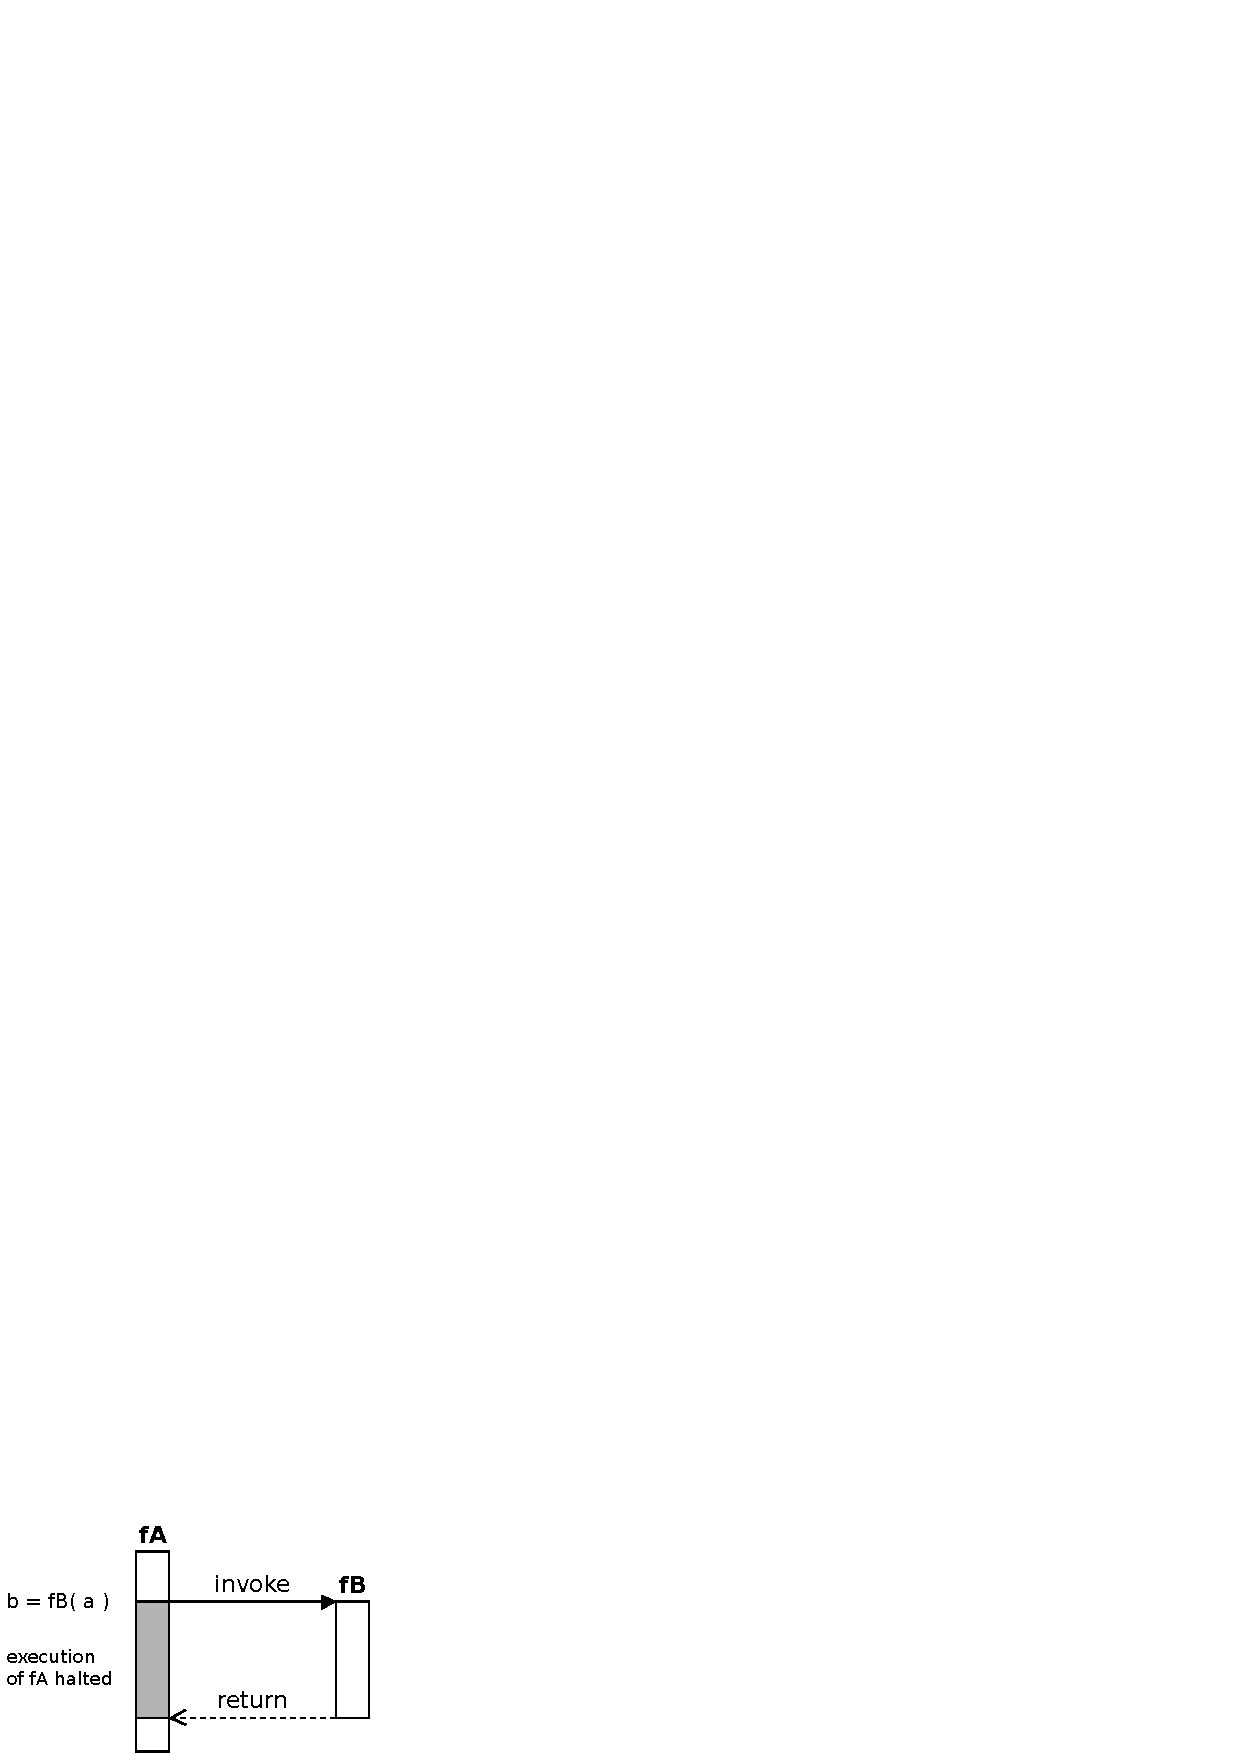
\includegraphics{figures/Closures_Synchronous}
	\caption{Synchronous Function Call}
	\label{fig:Closures_Synchronous}
\end{figure}

Asynchronous code execution, as shown in Figure~\ref{fig:Closures_Asynchronous}, allows non-blocking and thus scalable applications.
Non-blocking operations are a remedy for optimzed resource allocation and open up ways to overcome previously described unnecessary resource bindings.
Processing any kind of latency-driven I/O operation asynchronously ( e.g. filesystem access and socket communication ) exploits resources that would otherwise be bound while waiting for completion.
Such operations are processed and completed whenever required resources are available.
\begin{figure}[!ht]
	\centering
  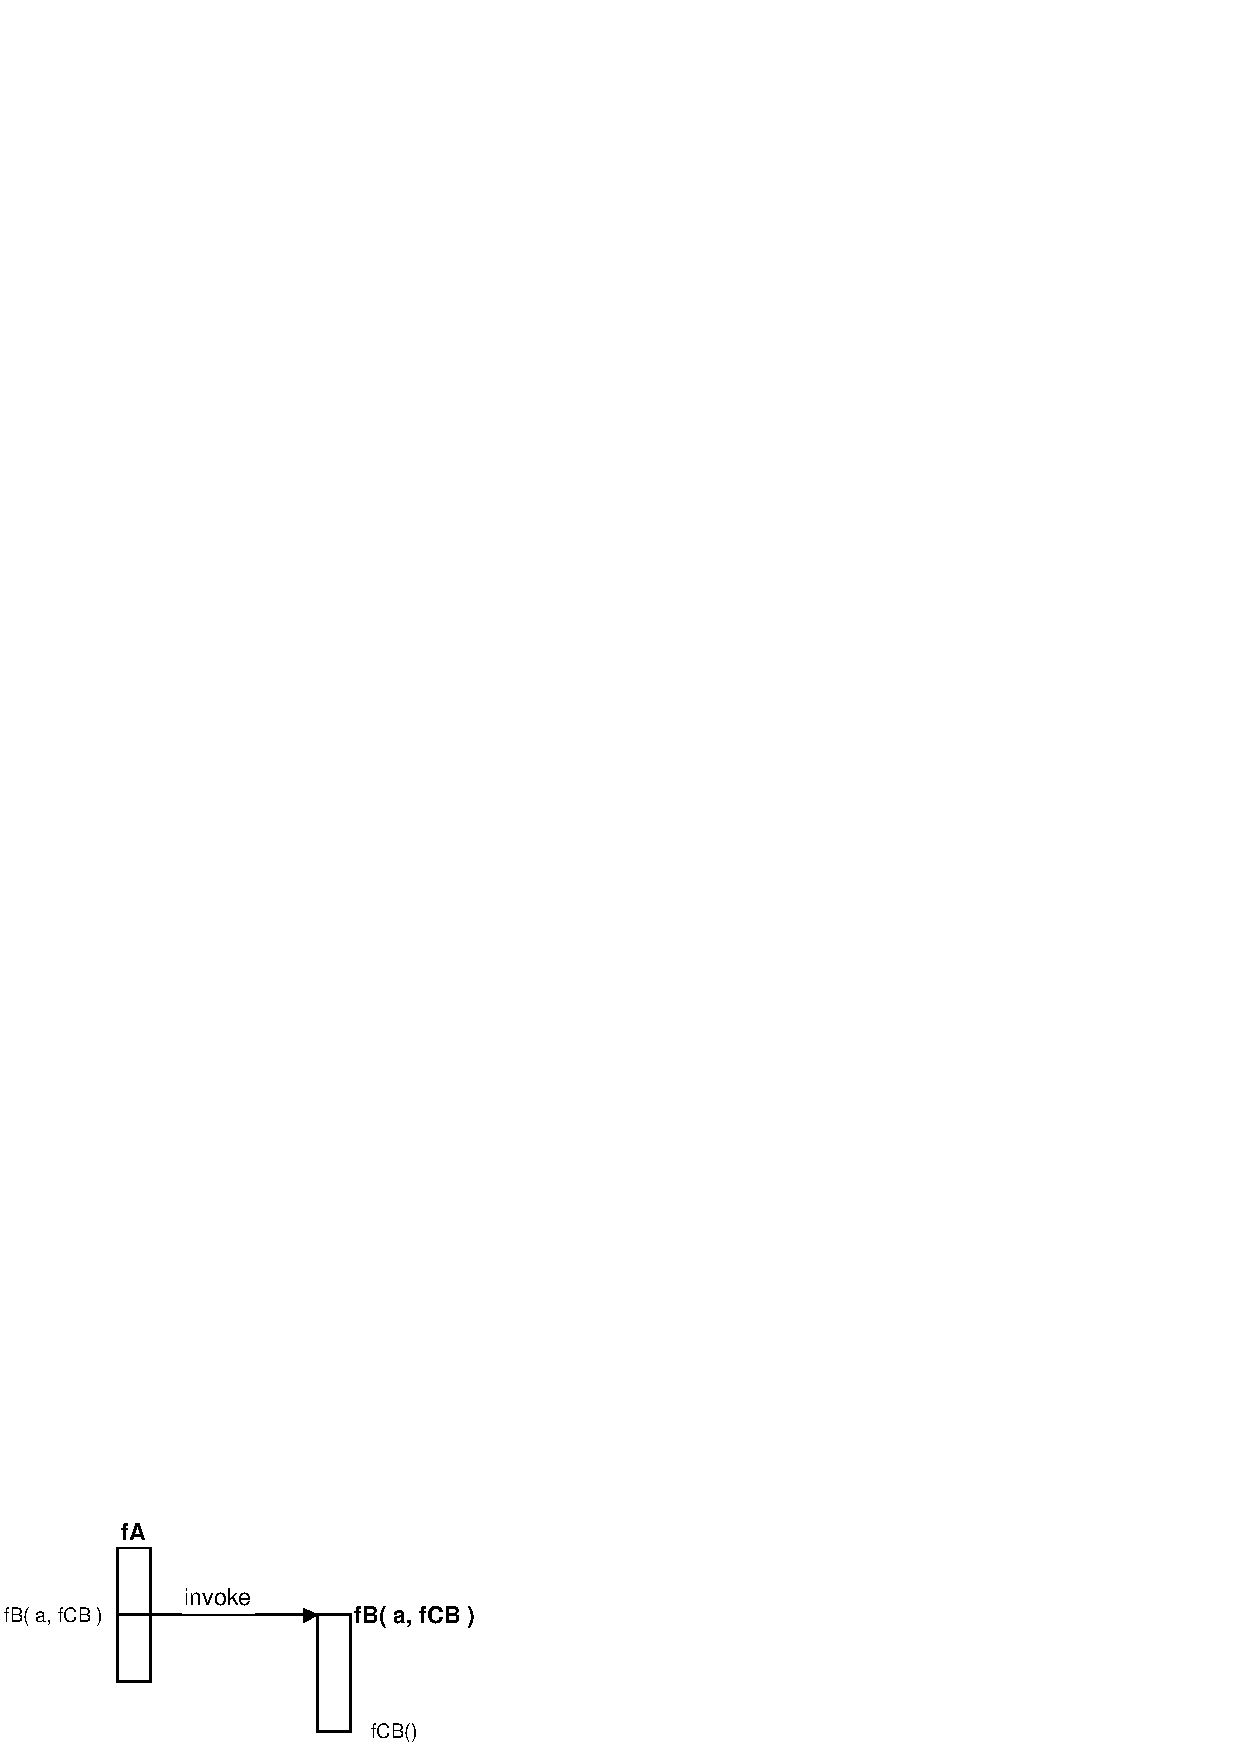
\includegraphics{figures/Closures_Asynchronous}
	\caption{Asynchronous Function Call}
	\label{fig:Closures_Asynchronous}
\end{figure}

Often other operations depend on the completion of asynchronous operations, hence their execution needs to be deferred.
This necessary code execution deferral is achieved through the use of callback functions, denoted \texttt{fCB} in Figure~\ref{fig:Closures_Asynchronous}.
Any code placed in a callback function, which is assigned to an asynchronous operation, is only executed after the respective asynchronous operation completed.
This allows stacking of functions and operations upon each other which automatically results in a flexible and event-driven application.

So far we didn't regard the context for such asynchronous functions.
If a function has access to the enclosing context where it was invoked in, it is called a closure.
Closures play an important role in ECMAScript\cite{EcmaScript}, which is the base for widely-spread script languages like JavaScript, JScript and ActionScript.
Closures in ECMAScript\cite{EcmaScript} are defined such as they have access to the context of the function they were created in.
This is shown in Figure~\ref{fig:Closures_Closure-1} where \texttt{c} from \texttt{fA}'s context is accessible from within \texttt{fB}, assuming that \texttt{fB} was created in \texttt{fA} and not only invoked from there.
Closures make it necessary for the context of the outer function to survive past its execution so no references are broken.
This is depicted through the "extended context lifetime" in Figure~\ref{fig:Closures_Closure-1}.
Using asynchronous closures it becomes evident, that the context in the invoking function can change while the closure is still computing and eventually referencing the outer context, thus causing race conditions.
This will be most obvious in a loop that immediately invokes \texttt{fB} several times, as shown in Figure~\ref{fig:Closures_Closure-2}.
In such a setup \texttt{c} will have different values in the same part of different invocations of \texttt{fB}.
\begin{figure}[!ht]
	\centering
  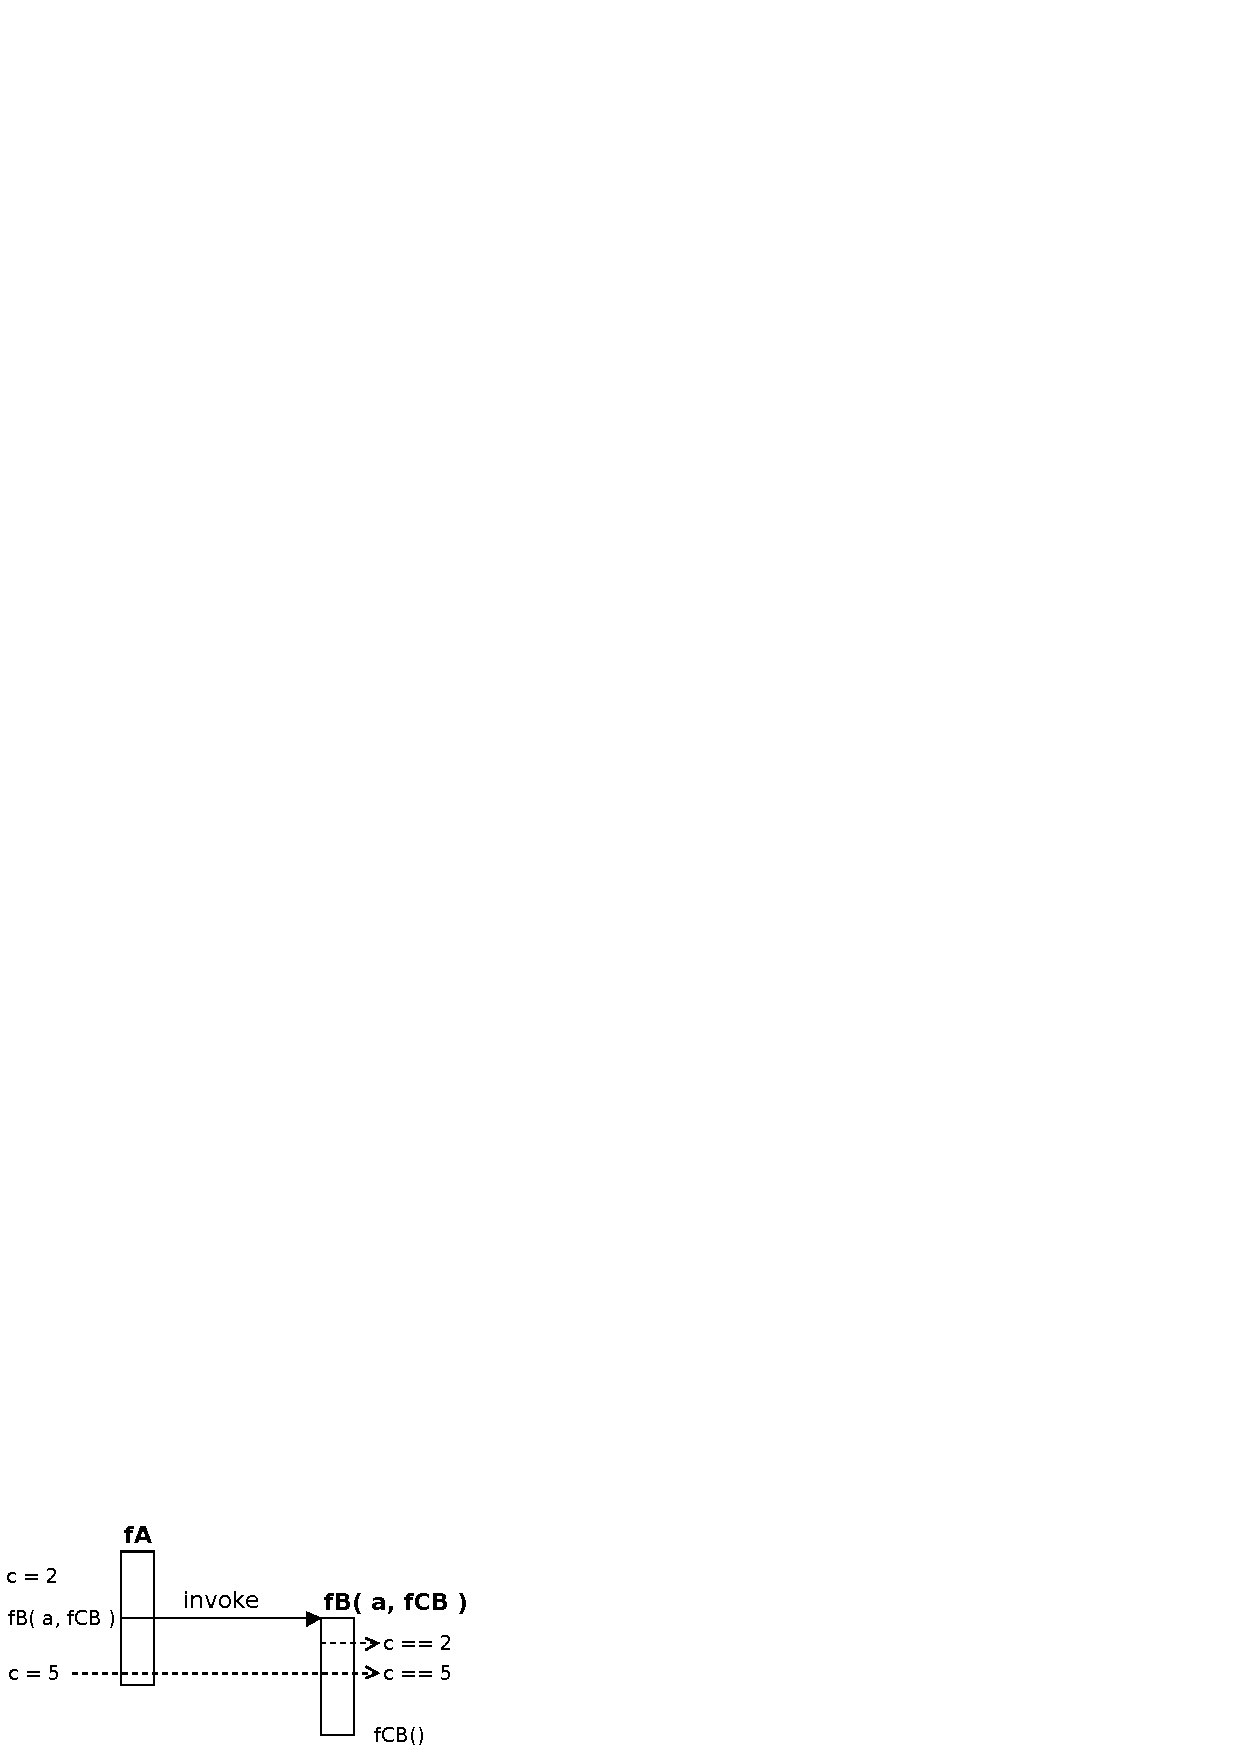
\includegraphics{figures/Closures_Closure-1}
	\caption{Closure Scope and referenced context}
	\label{fig:Closures_Closure-1}
\end{figure}
\begin{figure}[!ht]
	\centering
  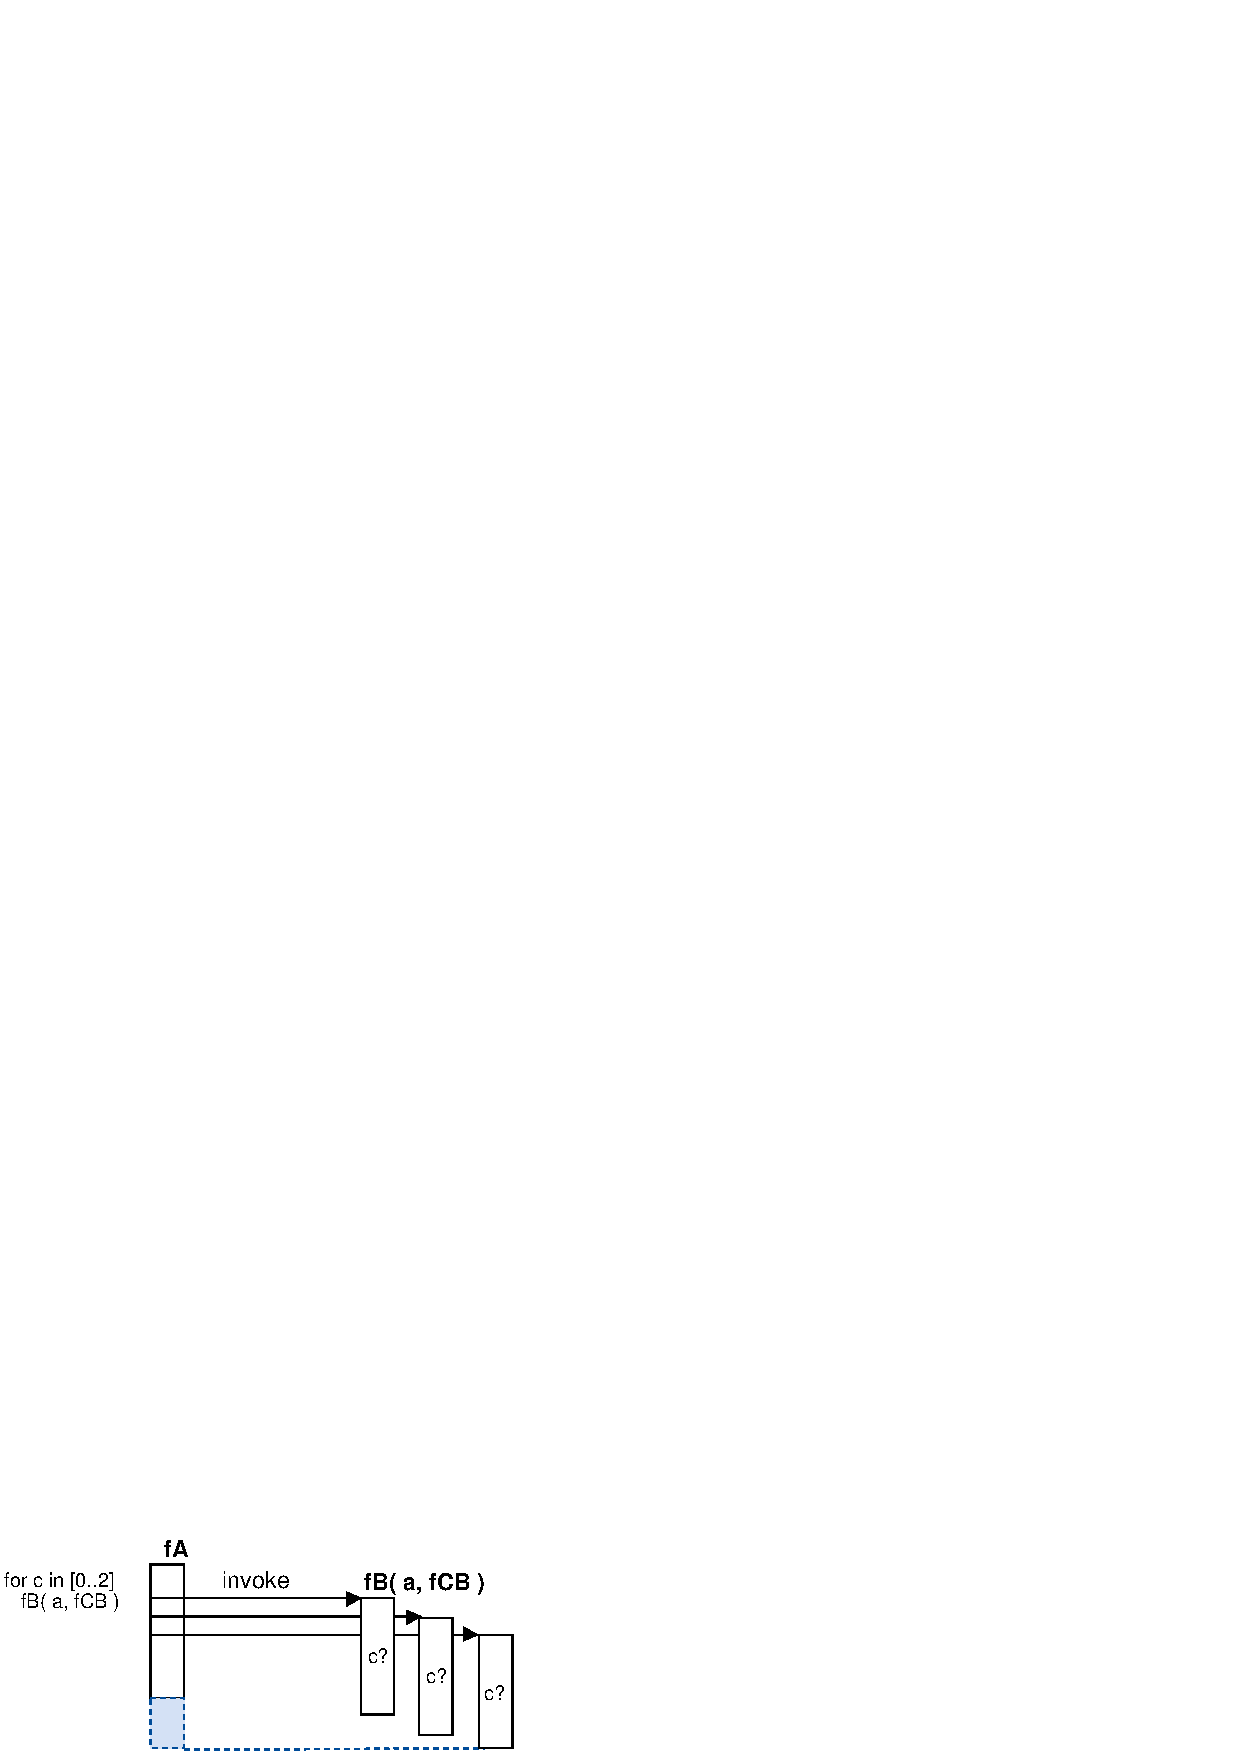
\includegraphics{figures/Closures_Closure-2}
	\caption{Closure context changes in a loop}
	\label{fig:Closures_Closure-2}
\end{figure}


Those event-driven context overwrites can be taken care of by shielding the closure from context changes, as shown in Figure~\ref{fig:Closures_Closure-3}.
To shield the closure form context changes, closure \texttt{fB} needs to create another closure \texttt{fC} and return it to \texttt{fA}.
The argument passed to \texttt{fB} is the context ( \texttt{c} in Figure~\ref{fig:Closures_Closure-3} ) that might change but requires to be persistent for one invocation.
\texttt{fC} has now \texttt{c} as a fixed context, which can't be overwritten anymore.
Now the only thing left is \texttt{fC} needs to be invoked and it will retain the original context.
This implementation is necessary when the closure acts as a callback function for asynchronous operations, to preserve the original context in case it is required within the callback function.
\begin{figure}[!ht]
	\centering
  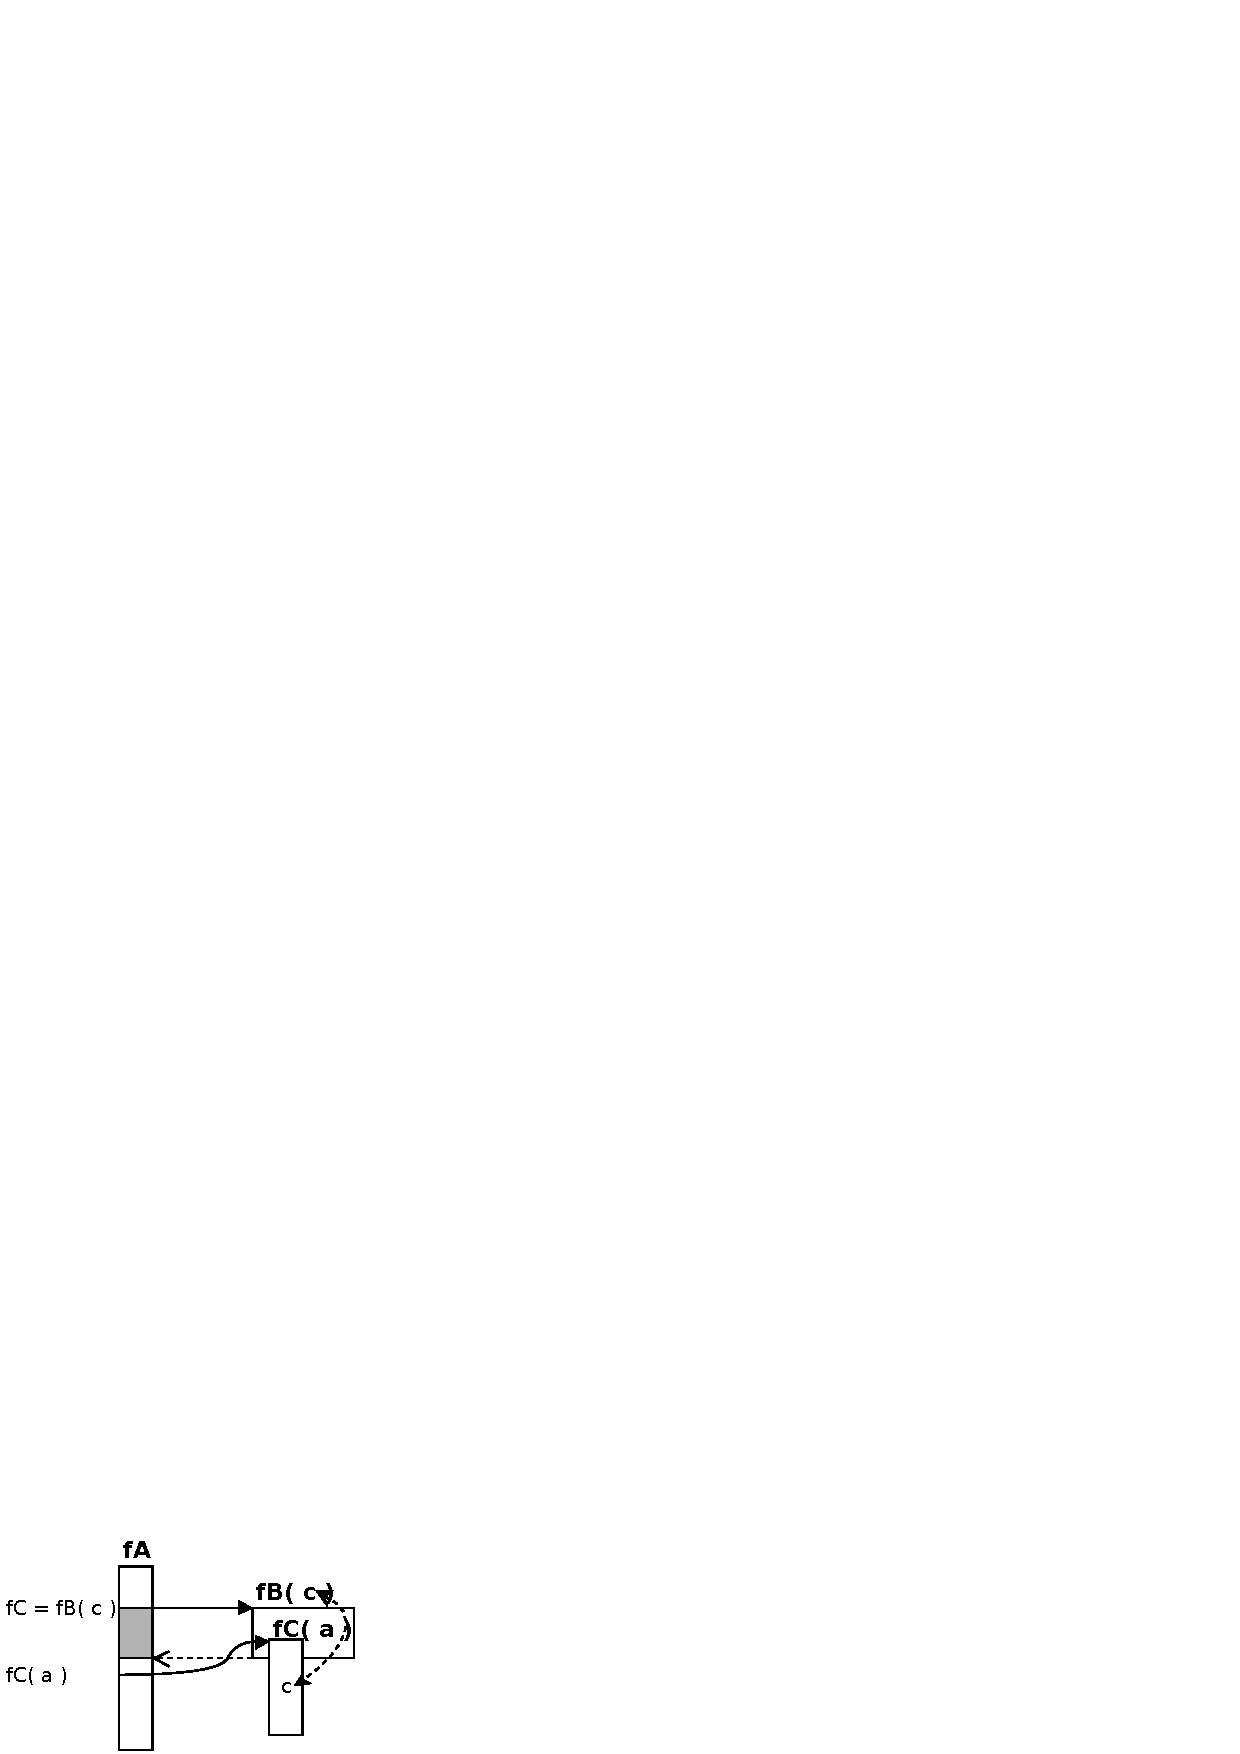
\includegraphics{figures/Closures_Closure-3}
	\caption{Closure Context Shielding}
	\label{fig:Closures_Closure-3}
\end{figure}

% TODO Figures need fA to be right aligned

An example of how closure contexts can be shielded is shown in the Listing \ref{lst_closure}.
\begin{lstlisting}[float=h,label=lst_closure,language=JavaScript,caption=JavaScript Context Shielding]
var fB = function( c ) { // Declare a function...
	var fC =  function( a ) { // ( <-- function to return )
		console.log( c );
	};
	return fC;
};
for( var c = 0; c < 100; c++ ) {
	// ... before you assign it to an event happening in the future:
	var fC = fB( c );
	setTimeout( fC, 3000); // will be executed after the loop ended
}
\end{lstlisting}

% TODO try async closures in other programming languages


% \subsubsection{Benchmarking JavaScript vs. Java}
% refer to listings
% TODO terminierungsproblem, testing, Web server, timeout, stacked callbacks.
%compilerbau?
%loesungsansätze?


% TODO why JS. JSON as first advantage (http://www.toptal.com/nodejs/why-the-hell-would-i-use-node-js)
% advantage for network applications with several concurrent connections
% not as client-server used as intented but as serverserver com since we also expect several connections simultanously under load.
% But also, we adopt the non-blocking nature of JS that is used for node's optimal communication, in order to implement our enigne in a non blocking way, thus allowing to load code and fire callback function in modules whenever they are required!
% http://ariya.ofilabs.com/2012/07/lazy-parsing-in-javascript-engines.html
% Optimization of special case if ( before function {immediately-invoked function expression (IIFE)}, do rela parsing, else lazy parsing
% Difference between context and scope. scope unique to each invocation, context is 'this', owner of currently executing code.
% .call, .apply 
% TODO we should use .bind for persistence.coffee's functions ....

%In JavaScript, functions are first-class objects, i.e. they are objects and can be manipulated and passed around just like any other object. Specifically, they are Function objects. -> https://developer.mozilla.org/en/docs/Web/JavaScript/Reference/Functions_and_function_scope
% Since each call provides potentially different arguments, a new closure is created for each call to outside. The memory can be freed only when the returned inside is no longer accessible

% The definitive guide: This combination of a function object and a scope (a set of variable bindings) in which the function’s variables are resolved is called a closure in the computer science literature.4
% This is an old term that refers to the fact that the function’s variables have bindings in the scope chain and that therefore the function is “closed over” its variables.


% Twelve Theses on Reactive Rules for the Web~\cite{10.1007-11896548_63}:
% This article investigates issues of relevance in designing high-level
% programming languages dedicated to reactivity on the Web. It presents
% twelve theses on features desirable for a language of reactive rules tuned
% to programming Web and Semantic Web applications.
% MY NOTES: they argue with soap and expect it to stay. They expect Web sites to inform each other about update requests. we are taking one step further and provide events to whomeever wants to receive them while being greedy about receiving events. give them to meeeeh my prciouzzz eventz!
% 1. High-level reactive languges are needed, ECA rules well-suited to specify reactivity
% 2. Reactive Web rules should be processed locally and act globally through event-based communication and access to persistent Web data
% 3. Events are best exchanged directly between Web sites in a push manner
% 4. Events are volatile data and should be kept distinct from persistent data.
% 5. Recognizing composite events is essential for a reactive Web language. Composite events are conveniently specified by (event) queries. There are (at least) four complementary dimensions to event queries: data extraction, event composition, temporal conditions, and event accumulation --> Future Work (CEP), data extraction already implemented
% 6. A data-driven, incremental evaluation of event queries is the approach of choice
% 7. Data from persistent Web resources plays an essential role for Web reactivity. A reactive language thus should embed or build upon a Web query language.
% 8. The Web is a dynamic, state-changing system. Reactions to state changes (events) through reactive rules are state-changing actions such as updates to persistent data. Reactive rules are needed where compound actions can be constructed from primitive actions.
% 9. Development and maintenance of reactive rule programs can be considerably supported by structuring mechanisms such as: branching in rules, deductive rules for event queries and Web queries, procedural abstractions for actions, and grouping of rules. --> Future work, attach several conditions and their actions branches to one event instead of creating rules for each of them. EC^nA^n. (Though procedural abstractions for actions already implemented, defining complex actions to be reused by rules)
% 10.Identity of data items is an issue for reactive languages due to their ability to react to changes of data objects on the Web. (we had surrogate identity though discarded the concept again... stupido)
% 11. Meta-programming and meta-circularity, that is, the ability to use rules to exchange and evaluate (other) rules, are needed in some important cases. (quite artificial for our scenarios)
% 12.Reactivity in the Web’s open and uncontrolled world requires language support for authentication, authorization, and accounting. (phew... let's let others go there)



% Tutorial example: as seen by user, as seen by the developer
